\documentclass[a4paper,11pt,openright,openbib]{article}
\usepackage[portuges]{babel}
\usepackage[T1]{fontenc}
\usepackage{ae}
\usepackage[utf8]{inputenc}
\usepackage[pdftex]{graphicx}
\usepackage{url}
\usepackage{listings}
\usepackage{verbatim}
\usepackage{enumerate}
\usepackage[a4paper, pdftex, bookmarks, colorlinks, linkcolor=black, urlcolor=blue]{hyperref} 
\usepackage[a4paper,left=2.5cm,right=2.5cm,top=3.5cm,bottom=3.5cm]{geometry}
\usepackage{colortbl}
\usepackage[margin=10pt,font=small,labelfont=bf]{caption}
\usepackage{mdwlist}


\setlength{\parindent}{0cm}
\setlength{\parskip}{2pt}




\title{
	\large{
\includegraphics[width=0.3\textwidth]{UM.jpg}} \\
	\large{Universidade do Minho}  \\
	\large{Mestrado em Engenharia Informática}  \\
	\large{Engenharia de Linguagens}  \\
	\large{Engenharia Gramatical - Grupo 1}  \\	
	\large{\textbf{Resolução da Avaliação 1}} \\
	\large{Ano Lectivo de 2012/2013} \\
	\date{\today}
}

\author{	
	\begin{tabular}[t]{c c}      
        pg22820 - \textbf{António Silva} \\        
		pg22781 - \textbf{Rui Brito} \\   				
	\\ 
	\end{tabular}
}

\begin{document}

\maketitle


\pagestyle{headings}
\pagenumbering{arabic}
\newpage
\tableofcontents
\newpage

\section{Introdução}
Neste documento é descrito o processo para a resolução da ficha de avaliação nº2. Tal como pedido no enunciado, foi implementada uma gramática para processar ficheiros .ma. Posteriormente foram adicionados atributos para a detecção de erros e de warnings, bem como contadores dos estados inicias, finais, instáveis, de transição... Por fim, através de classes fornecidas pelo docente, o ficheiro .ma foi convertido para o formato dot.

\section{Resolução} % (fold)
\label{sec:resolucao}

\subsection{Gramática} % (fold)
\label{sub:gram_tica}

Numa fase inicial, e depois de interpretarmos os requisitos da linguagem, implementamos uma gramática em \emph{ANTLR}.
A regra \emph{root} é a seguinte:
\small
\begin{verbatim}
	imc	:	
    INITIAL_STATE a=state[""]+ FINAL_STATE b=state[""]+ TRANSITION_STATE transitions+;
\end{verbatim}

A regra apresentada acima, serve para ter uma ideia do contorno geral da gramática. Para não sobrecarregar este relatório, tomamos a decisão de não incluir a gramática na integra, pelo que ela é fornecida no zip em que também vai este relatório. Para dar uma ideia do código implementado, segue abaixo a implementação das transições, já com os atributos.

\normalsize
% subsection gram_tica (end)

\subsection{Detecção de Erros e Warnings} % (fold)
\label{sub:detec_o_de_erros_e_warnings}
Nesta fase da resolução procedemos à introdução de atributos na gramática para o tratamento de erros e avisos. 

\small
\begin{verbatim}
   transitions:	st=state[""] {	
       if (!states.add($st.actual_st)) {    	
       System.out.println("ERROR (multiple definitions of state " + $st.actual_st + "): " + 
                                        "line -> " + $st.line + " column -> " + $st.pos);
        }					
   }	
   (ac=action|mt=markovian_trans) {    	 
       if(mt == false) {		 
           if($ac.action_value.equals("tau")) {		
               System.out.println("Warning (source is unstable state): " + "line -> "
                                           + $st.line + " column -> " + $st.pos);        	
           }
       }    	
   }	 	
   transition_def[$markovian_trans.isMarkovian, $action.isAction,$state.actual_st]+;
\end{verbatim}
\normalsize

Como pode ser visto acima, sempre que um erro é detectado, faz-se simplesmente um \emph{println()}. Pode também ver-se, que não só erro, mas também a linha a coluna onde esse erro acontece são mostrados no ecrã, de forma a facilitar a vida do utilizador final. 
% subsection detec_o_de_erros_e_warnings (end)

\subsection{Contador de estados} % (fold)
\label{sub:contador_de_estados}
Nesta fase da resolução, dado que o projecto já estava a ficar grande demais para implementar apenas em \emph{ANTLR} decidimos implementar as nossas classes para o efeito desta alínea em separado, optando por incluir o processador no projecto. Decidimos também implementar um classe para os erros, tornando-os disponíveis a partir de métodos get do java, bem como uma distinção entre os tipos de erros. \\
Essa distinção é feita a partir de um \emph{enum}.
\small
\begin{verbatim}
public enum error_type {
        WARNING,
        ERROR
    }	
\end{verbatim}
\normalsize
Os erros estão contidos num HashSet<Error> sendo Error uma classe privada à classe IMC\_Error. Posteriormente, foi feita a classe IMC\_Info, onde está incluida uma instância da classe IMC\_Error, bem como os vários contadores pedidos nesta alínea.
Para contar estes estados, alteramos o parser e o lexer gerados pelo \emph{ANTLR}. As alterações foram simples, por exemplo, para calcular os estados iniciais, finais e de transição, introduzimos o seguinte código:
\small
\begin{verbatim}
    (...)
    Token st2=null;		

    try {						
        st2=(Token)match(input,ID,FOLLOW_ID_in_state178);
    {
        if(IMCLexer.isInitial) {
	        info.incInitStates();				
        }
        if(IMCLexer.isFinal) {		
            info.incFinalStates();				
        }
        if(IMCLexer.isTransition) {				
	        info.incTransStates();				
        }
        (...)
    }			
\end{verbatim}
\normalsize
Foram introduzidas variaveis protected na classe IMCLexer para saber em que ponto estamos da gramática e depois apenas usamos métodos da classe IMC\_Info, instaciada na classe do parser para incrementar os valores.
% subsection contador_de_estados (end)

\subsection{Objecto IMC} % (fold)
\label{sub:todotformat}
Esta talvez tenha sido a alínea mais complexa, pois foi preciso ir a um nível de detalhe em que era necessária muito minunciosidade, mas sempre sem perder a noção geral do código.\\
Assim, tal como anteriormente, começamos por instanciar a classe IMC (fornecida pelo docente). De seguida, foram identificados os pontos onde seria necessário colectar informação. O código continua a ser bastante simples, mas foi bastante complicado identificar onde ele deveria estar. Por exemplo, o código para identificar o nó de origem é o seguinte.
\small
\begin{verbatim}
    (...)
    try {
        {
            pushFollow(FOLLOW_state_in_transitions70);
            st=state("");			
            
            imc.addState(st.start.getText());
            startS = st.start.getText();
            (...)            
\end{verbatim}
\normalsize
De notar que neste exemplo também é possível ver como foram adicionados os estados à lista. \\
Quanto à inserção do objecto, esta é feita assim que é possível, ou seja, na regra que faz match aos números referentes à taxa ou probabilidade de transição. Ou seja, na regra \emph{trans\_prob\_rate}.
\small
\begin{verbatim}
    a=(Token)match(input,FLOAT,FOLLOW_FLOAT_in_trans_prob_rate133); 				
        if(isA) 
	            imc.addTransition(new InteractiveTransition(startS,goalS,action));					
        if(isM)
	            imc.addTransition(new MarkovianTransition(startS, goalS, Double.parseDouble(
	                                            a.getText())));
\end{verbatim}
\normalsize
Por fim, e como pedido no enunciado, foi usado o método \emph{toDotFormat()} da classe IMC fornecida, o output do mesmo é o seguinte:
\begin{figure}[!htp]
	\centering	
		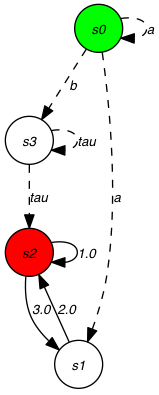
\includegraphics[scale=0.7]{dotIMC.png}		
\end{figure} 
% subsection todotformat (end)

% section resolu_o (end)


\section{Conclusão}
Após a resolução desta ficha de avaliação, julgamos que todos os objectivos foram cumpridos com sucesso. De uma forma geram a ficha foi fácil de resolver, houveram alguns pequenos contratempos, mas nada que comprometesse os resultados finais. 
\end{document}
